% !TEX root = ../thesis.tex

\chapter{Research Methodology and Design} \label{chp:methodology}

\section{Overall Research Design and Technical Framework}

This research adopts a systematic and progressive research design that aims to systematically address three core research questions through technical innovation, methodological contributions, and empirical validation, thereby constructing a comprehensive solution. The overall technical framework embodies a complete chain from theoretical construction to technical implementation, then to clinical validation and application translation, ensuring that each research component has clear objectives, scientific methods, and measurable outcomes.

\begin{figure}[htbp]
\centering
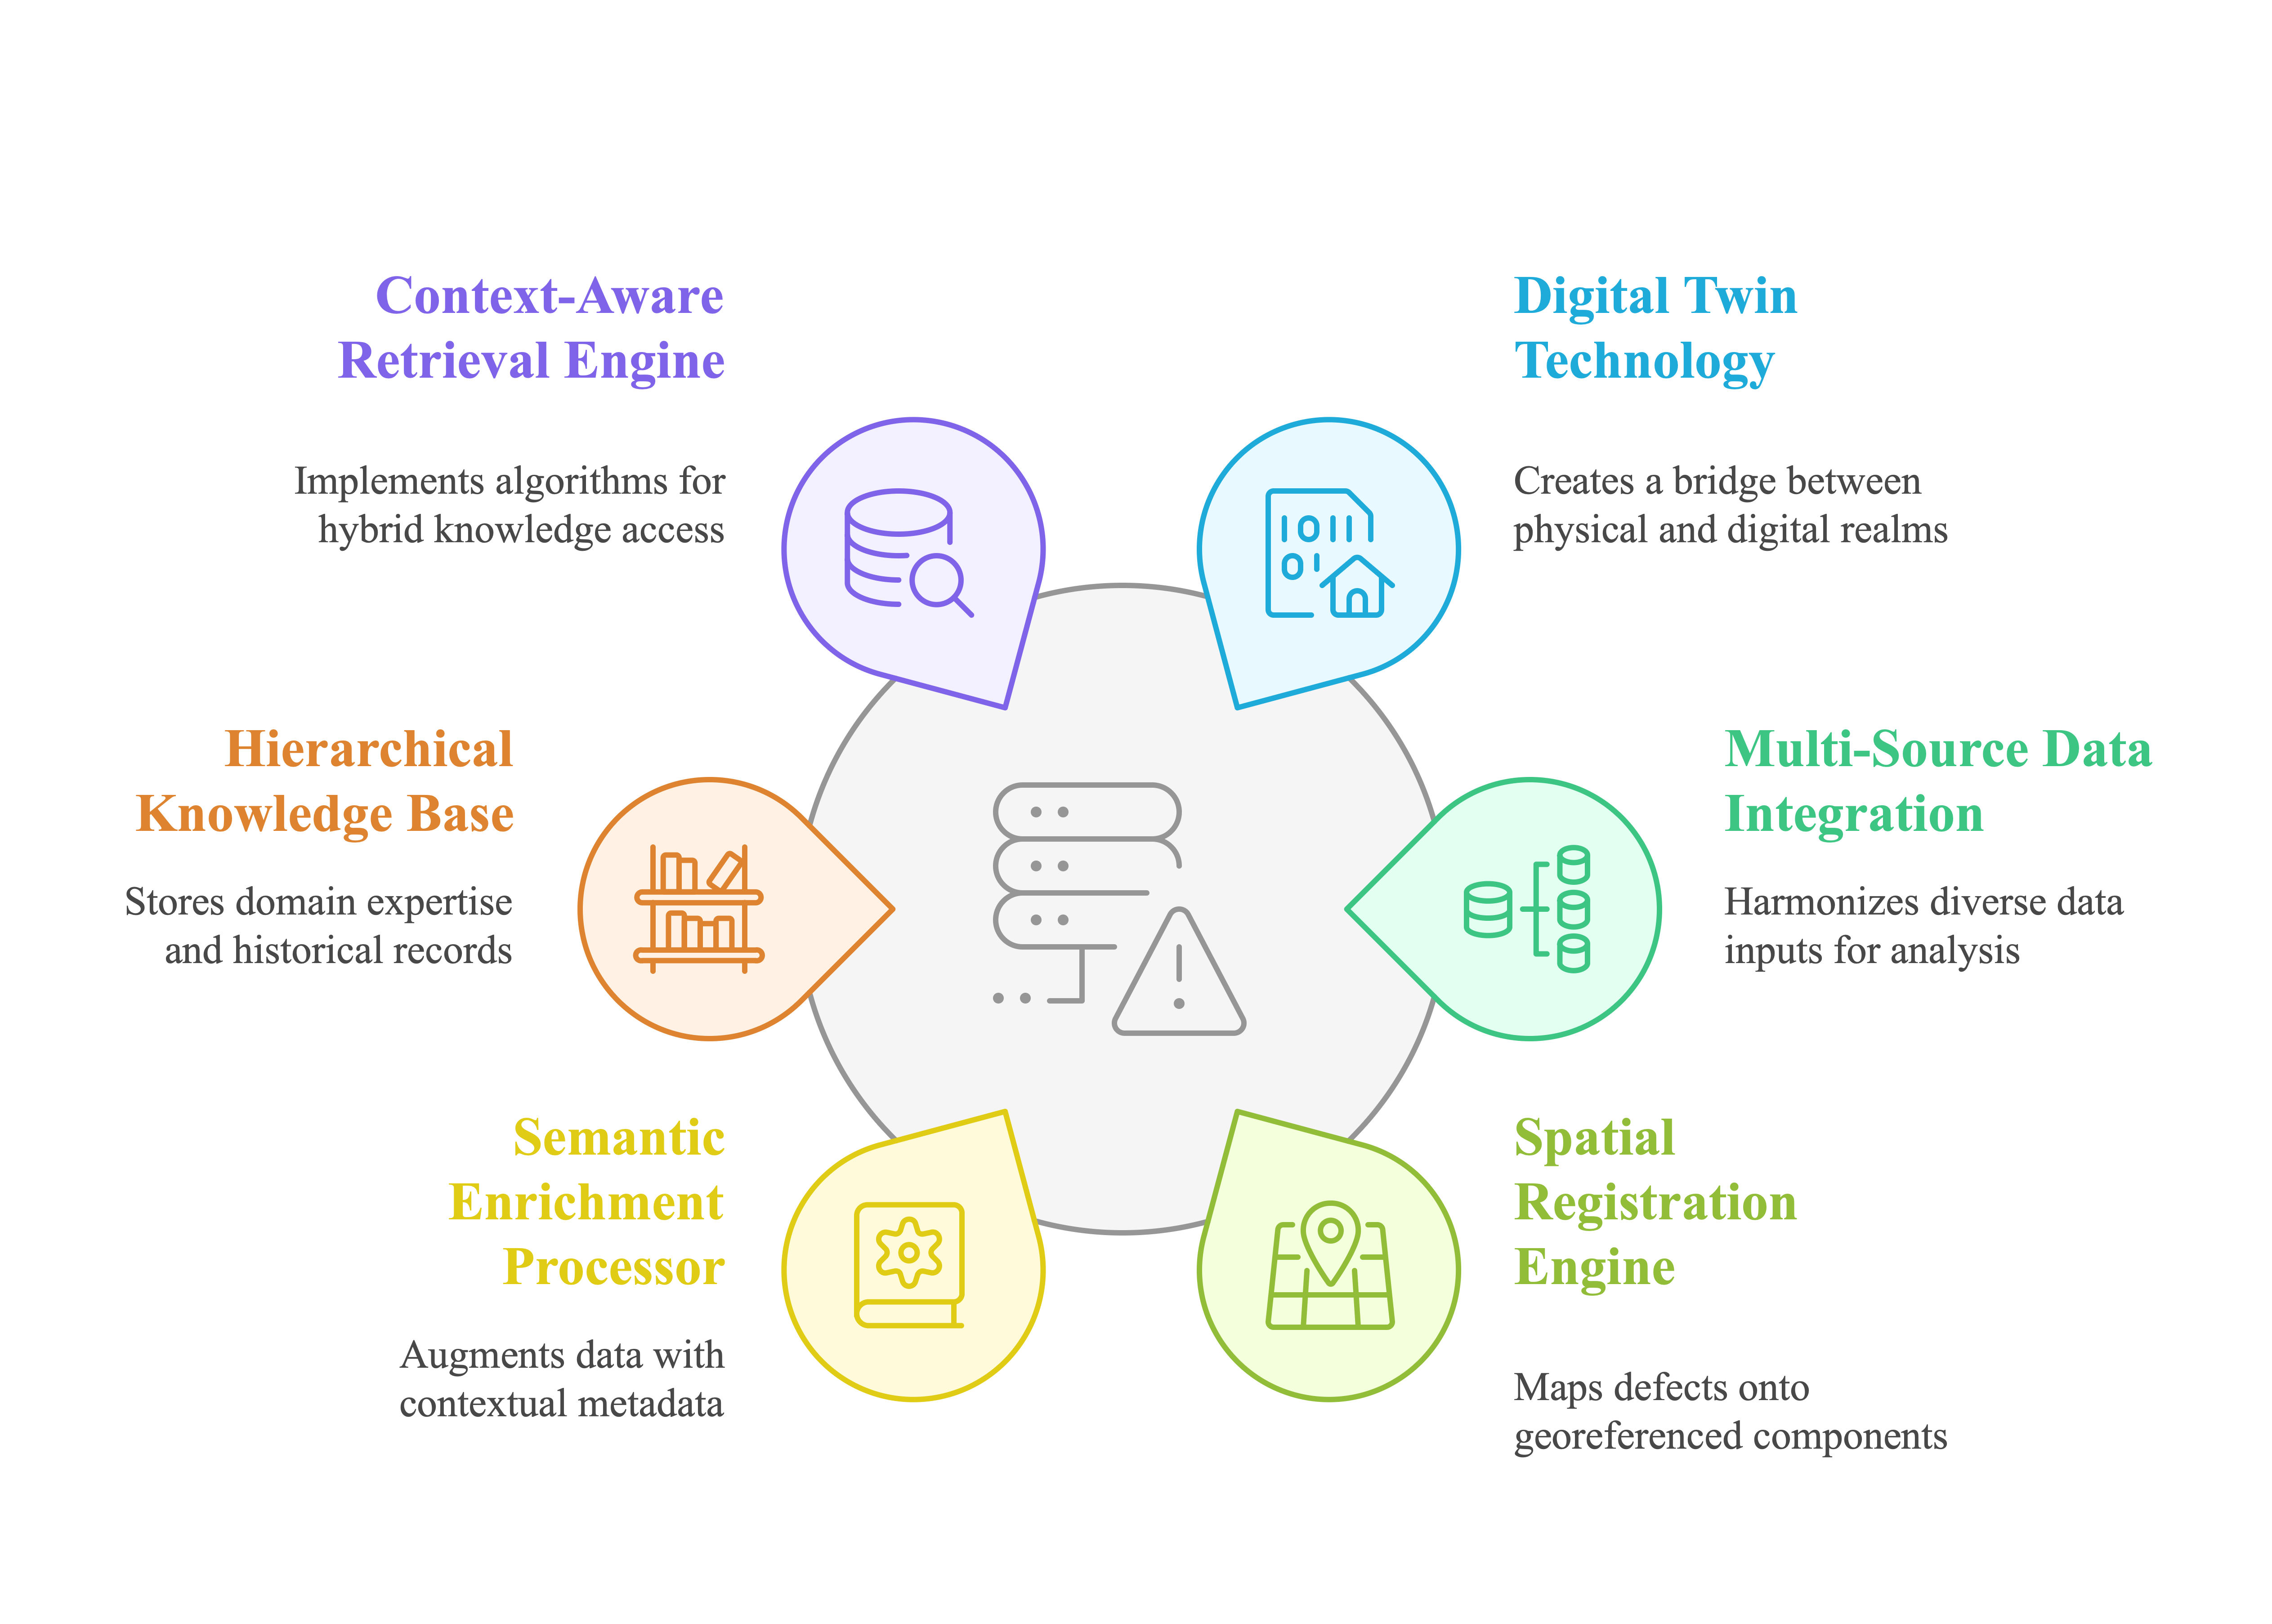
\includegraphics[width=0.9\textwidth]{DefectGPT/Overall_Framework.png}
\caption{Overall technical framework diagram showing the logical relationships between three research questions, research objectives, and specific research content}
\label{fig:overall_framework}
\end{figure}

The technical framework design follows the scientific research paradigm of "problem-oriented - solution - validation and evaluation." Addressing Research Question 1 concerning the construction of unified computational frameworks, the research will proceed from theoretical analysis based on the "Four Pillars of Synergy" theory, designing and implementing the USANet unified framework through a "Two-Stage Knowledge Injection" training strategy to achieve synergistic learning for gastric and pancreatic cancer assessment tasks. For Research Question 2 regarding clinical trust and value validation, the research will establish a multi-dimensional validation system that transcends traditional technical metrics, ensuring that the clinical value of the AI framework receives scientific and rigorous validation through comprehensive assessment across technical performance, clinical endpoint correlation, and decision-making value dimensions.

Addressing Research Question 3 concerning seamless clinical workflow integration, the research will design and develop the Sono-Agent human-AI collaborative workflow prototype through real-time dynamic scanning assistance and knowledge-enhanced intelligent report generation, exploring deep integration of AI technology in ultrasound diagnostic workflows. The entire research design emphasizes the combination of theory and practice, the alignment of technical innovation with clinical needs, ensuring that research outcomes possess both academic value and practical application prospects. This comprehensive approach recognizes that successful medical AI development requires not only technical excellence but also deep understanding of clinical context and practical implementation requirements.

\section{Dataset Construction and Ethical Considerations}

\subsection{Data Sources and Collection Standards}

This research will construct a high-quality, large-scale multi-center gastric and pancreatic cancer transabdominal ultrasound dataset, serving as the foundation for unified framework training and validation. Data collection will adopt a multi-center retrospective study design, planning to collaborate with five to eight tertiary hospitals domestically and internationally that possess extensive ultrasound diagnostic experience, including multiple departments such as gastroenterology, oncology, and ultrasound departments. This multi-center design ensures data representativeness and diversity, effectively reducing potential bias from single-center data and enhancing model generalization capabilities.

The data collection time window is set from January 2018 to December 2023, ensuring data timeliness while accumulating sufficient case numbers. Collection standards will strictly adhere to ethical guidelines and data quality requirements for medical research, ensuring legality, accuracy, and completeness of all data. Participating medical institutions will undergo rigorous selection based on case volume, technical capabilities, and data quality to ensure overall dataset quality. The collaborative approach recognizes that ultrasound expertise varies significantly across institutions and that data diversity is essential for developing robust AI systems that can generalize across different clinical settings and patient populations.

\subsection{Gastric Cancer Dataset Specifications}

Construction of the gastric cancer dataset will follow strict inclusion and exclusion criteria to ensure data quality and clinical relevance. Inclusion criteria encompass patients aged 18-80 years, pathologically confirmed gastric cancer patients or benign lesion patients confirmed through long-term follow-up of at least two years, complete transabdominal ultrasound examination records including static images and dynamic videos, ultrasound examination to pathological diagnosis interval not exceeding 30 days, and complete clinical data including TNM staging, treatment protocols, and follow-up results. These criteria ensure that the dataset captures clinically relevant cases with sufficient diagnostic certainty and temporal proximity between imaging and pathological confirmation.

Exclusion criteria include excessively poor image quality preventing effective assessment, concurrent other abdominal malignancies, preoperative neoadjuvant chemotherapy or radiotherapy, and incomplete clinical data or lost follow-up. Based on preliminary research and sample size calculations, the gastric cancer dataset targets collection of 2000-3000 cases, with malignant cases comprising 60-70% and benign cases 30-40%. Image types will include standardized static images in DICOM format and dynamic scanning videos in MP4 or AVI format, with each case containing at least 10-15 key static images and 2-3 dynamic video segments. This comprehensive imaging approach captures both detailed morphological information and functional characteristics that are crucial for AI model training and validation.

\subsection{Pancreatic Cancer Dataset Specifications}

Pancreatic cancer dataset inclusion criteria are similar to gastric cancer but pay special attention to pancreatic cancer specificities. Inclusion criteria encompass patients aged 18-85 years, pathologically confirmed pancreatic cancer patients or benign pancreatic lesions confirmed through imaging and clinical follow-up, transabdominal ultrasound capable of clearly displaying the pancreas with image quality meeting assessment requirements, complete CT or MRI comparative data, and complete clinical staging and treatment information. Considering the relative rarity of pancreatic cancer and technical difficulties in transabdominal ultrasound pancreatic observation, pancreatic cancer dataset collection will emphasize quality control even more stringently.

Exclusion criteria include unclear pancreatic display or complete obstruction by intestinal gas, chronic pancreatitis and other benign diseases severely affecting pancreatic morphology, and special tumor types such as pancreatic endocrine tumors. The target collection for the pancreatic cancer dataset is 1500-2500 cases with approximately equal malignant to benign ratios. Due to the specificity of pancreatic ultrasound examination, data will particularly include images from different positions such as supine and lateral positions and different hydration states including fasting and post-water drinking to maximize pancreatic visualization effectiveness. This approach recognizes the technical challenges specific to pancreatic imaging and the need for comprehensive scanning protocols to overcome anatomical limitations.

\subsection{Data Annotation Protocols}

Data annotation represents the critical component ensuring dataset quality, and this research will establish a rigorous multi-level annotation and quality control system. The annotation team will comprise 10-15 experts holding associate chief physician level or above with more than 10 years of ultrasound diagnostic experience from different hospitals, including specialists dedicated to digestive system ultrasound diagnosis. Annotation work will be organized into three levels: primary annotation, cross-review, and expert final review. This hierarchical approach ensures both efficiency and accuracy while maintaining consistency across different annotators and institutions.

Annotation content will include lesion bounding box annotation using standard rectangular boxes to mark suspicious lesion positions and ranges, precise segmentation masks providing pixel-level segmentation annotation for definite lesions, benign-malignant classification annotation based on morphological features providing probability assessments, and key imaging feature annotation including echo characteristics, boundary features, blood flow signals, and relationships with surrounding structures as clinical diagnostic elements. Each case will receive independent annotation from at least three different physicians, with annotation consistency quantified through Kappa values. Cases with low consistency will undergo expert consultation to determine final annotations. This comprehensive annotation approach ensures that the dataset captures the full spectrum of diagnostic features while maintaining inter-observer reliability.

\subsection{Data Anonymization and Ethical Approval}

Data privacy protection and ethical compliance constitute important components of this research. All collected medical data will be processed strictly according to relevant laws and regulations including the Personal Information Protection Law and Data Security Law. The data anonymization process will include removal of all direct identifying information such as names, identification numbers, and contact information, de-identification processing of indirect identifying information such as replacing birthdates with age ranges and addresses with regional codes, and technical processing of imaging data to remove DICOM tags that may contain patient information.

This research will submit detailed research protocols to ethics committees of participating hospitals before beginning data collection to apply for ethical approval. Ethical approval will cover research scientific validity, necessity, risk assessment, data usage scope, and data security measures. For retrospective studies, ethical exemption from informed consent will be requested while establishing strict data usage supervision mechanisms. Additionally, data security management systems will be established including data access permission control, data transmission encryption, and data storage security measures to ensure adequate patient privacy protection. These measures reflect contemporary standards for responsible medical data research and ensure compliance with evolving privacy regulations.

\section{Research Content One: Construction of Unified Computational Framework}

\subsection{Theoretical Foundation Based on Multi-task Learning and Representation Disentanglement}

The theoretical foundation for constructing the unified framework in this research derives from two core ideas in machine learning: Multi-Task Learning (MTL) and Representation Learning. The core concept of MTL is that by having a model simultaneously learn multiple related tasks, it can utilize shared information between tasks, enabling the model to learn more generalizable feature representations and thereby improve performance on individual tasks. This aligns perfectly with the "Four Pillars of Synergy" theory of this research, where gastric and pancreatic cancer assessment tasks represent precisely such a group of intrinsically related tasks.

However, simply sharing an encoder for multi-task learning may lead to "negative transfer" or gradient conflict problems between tasks. Therefore, this research will further introduce the concept of representation disentanglement. The goal is to have different parts of the learned feature vectors correspond to different, interpretable sources of variation. For example, some features might encode universal organ anatomical structures representing task-shared information, while other features encode specific lesion attributes representing task-specific information. Through this approach, we aim to maximize positive synergy between tasks while minimizing mutual interference, thereby achieving more efficient and robust synergistic learning. This theoretical framework provides a principled approach to balancing shared learning with task-specific requirements.

\subsection{Core Methodology: Two-Stage Knowledge Injection Training Strategy}

To translate the above theory into a practically feasible training pipeline, this research designs a novel "Two-Stage Knowledge Injection" training strategy. The core of this strategy lies in mimicking the learning process of human physicians, first learning general anatomical knowledge, then learning specific disease diagnostic knowledge. This biomimetic approach recognizes that effective medical AI systems must first understand normal anatomy before learning pathological variations.

The first stage involves general abdominal representation pre-training. In this stage, we do not require large amounts of finely annotated cancer data. Instead, we will utilize large-scale, weakly labeled or even completely unlabeled abdominal ultrasound video data collected from multiple centers. Through self-supervised learning methods such as contrastive learning approaches like MoCo and SimCLR or masked image modeling like MAE, we force the model to learn universal, intrinsic visual patterns and anatomical structures in abdominal ultrasound imaging. The product of this stage is a powerful visual encoder that, like a student who has studied anatomy, possesses deep understanding of the basic "grammar" of the abdomen.

The second stage involves multi-task knowledge joint fine-tuning. In this stage, we will "freeze" or fine-tune with smaller learning rates the encoder pre-trained in the first stage, loading multiple task-specific heads designed specifically for gastric and pancreatic cancer assessment tasks on top of it. We then use high-quality, precisely annotated gastric and pancreatic cancer datasets to jointly train these task heads and optionally the upper layers of the encoder. This process is equivalent to having a student who already understands anatomy begin studying tumor diagnostics. Because the encoder already possesses powerful general representation capabilities, the second-stage fine-tuning process becomes more efficient and stable, and can better utilize precious, gold-standard annotated data, thereby precisely "injecting" disease-specific diagnostic knowledge into the model.

\subsection{Model Architecture: Unified Sonographic Assessment Network}

USANet (Unified Sonographic Assessment Network) represents the core technical implementation of the unified deep learning framework proposed in this research. The network design fully considers the special properties of ultrasound images and multi-task learning requirements, adopting an advanced hybrid architecture design that balances multiple competing objectives while maintaining computational efficiency and clinical interpretability.

The backbone design of USANet employs advanced CNN-Transformer hybrid architectures, specifically adopting ConvNeXt or MaxViT as encoders. This design can balance local texture feature extraction and global context modeling capabilities. CNN components are responsible for extracting detailed texture information from ultrasound images, crucial for identifying subtle lesion features such as echo patterns and boundary characteristics. Transformer components capture global anatomical relationships through self-attention mechanisms, effectively modeling spatial relationships between stomach and pancreas as well as interactions between lesions and surrounding structures. This hybrid approach leverages the complementary strengths of both architectural paradigms while addressing the unique requirements of ultrasound image analysis.

The task heads design builds upon the unified encoder with USANet designing four specialized task heads to handle different assessment tasks. The Localization Head, based on structures similar to YOLO or DETR, outputs lesion bounding boxes and can simultaneously detect suspicious lesions in both stomach and pancreas while providing precise location information. The Segmentation Head, based on structures similar to U-Net, outputs pixel-level segmentation masks and can perform precise contour delineation for detected lesions, providing foundation for subsequent morphological analysis. The Classification Head performs global average pooling on encoded features and outputs benign-malignant probabilities through fully connected layers, integrating full-image information to provide overall diagnostic judgments. The Attribute Assessment Head consists of multiple parallel classification and regression heads for evaluating imaging features strongly correlated with TNM staging, such as assessing signs of serosal invasion for gastric cancer or vascular encasement relationships for pancreatic cancer.

\subsection{Loss Function Design and Optimization Strategy}

To effectively train the multi-task network, this research designs a weighted composite loss function that balances multiple objectives while ensuring stable convergence. The total loss function is formulated as: $L_{total} = w_1 L_{loc} + w_2 L_{seg} + w_3 L_{cls} + w_4 L_{attr}$, where each component addresses specific task requirements. The localization loss $L_{loc}$ adopts Focal Loss or GIoU Loss to handle class imbalance problems in object detection. The segmentation loss $L_{seg}$ uses a combination of Dice Loss and Cross-Entropy Loss to ensure both boundary accuracy and region completeness. The classification loss $L_{cls}$ employs weighted Cross-Entropy Loss to handle benign-malignant sample imbalance. The attribute assessment loss $L_{attr}$ selects appropriate loss functions based on specific attribute characteristics.

The weight parameters $w_1, w_2, w_3, w_4$ will be determined through experimentation, with research into dynamic weight adjustment strategies such as Uncertainty Weighting or GradNorm methods to balance learning progress across different tasks and prevent any single task from dominating the training process. This adaptive approach ensures that all tasks receive appropriate attention during training while accommodating the different convergence rates and optimization landscapes of different objectives. The loss function design reflects contemporary best practices in multi-task learning while addressing the specific challenges of medical image analysis.

\subsection{Experimental Design and Comparative Analysis}

To comprehensively evaluate USANet performance, this research will design rigorous comparative experiments that isolate the contributions of different components and training strategies. Comparative baselines will include multiple "single-task, single-model" specialized networks trained separately for gastric cancer detection, pancreatic cancer detection, benign-malignant classification tasks, simple multi-task networks without the "Two-Stage Knowledge Injection" strategy, and existing medical image analysis networks such as ResNet and DenseNet widely used in medical imaging.

Ablation studies will systematically verify the effectiveness of various components through controlled experiments. These studies will verify the effectiveness of the "Two-Stage Training Strategy" through comparison with end-to-end training, validate the advantages of "multi-task joint learning" through comparison with single-task learning, verify the contributions of different architectural components such as CNN versus Transformer and different attention mechanisms, and validate the reasonableness of loss function design through different weight settings and loss function combinations. This comprehensive experimental design ensures that claims about the benefits of the unified approach are supported by rigorous empirical evidence and that the individual contributions of different innovations can be properly attributed.

\section{Research Content Two: Establishment of Multi-dimensional Comprehensive Validation System}

\subsection{Technical Performance Validation}

Technical performance validation constitutes the foundational level of AI model assessment, aiming to comprehensively evaluate USANet technical metric performance across specific tasks. Validation will be conducted on independent test sets sourced from medical institutions different from training sets to ensure evaluation objectivity and generalizability. This approach recognizes that technical performance, while necessary, is insufficient for establishing clinical utility and must be complemented by higher-level validation approaches.

For classification tasks, key indicators will be evaluated including accuracy reflecting overall diagnostic correctness, precision and recall separately assessing model ability to identify positive cases and coverage capability, F1 score providing harmonic mean of precision and recall, and AUC value assessing comprehensive performance under different thresholds with detailed ROC curve visualization analysis. Particularly, DeLong tests will be used to compare AUC differences between different models for statistical significance, ensuring statistical reliability of performance improvements. This statistical rigor ensures that observed differences reflect genuine improvements rather than random variation.

For segmentation tasks, standard indicators from medical image segmentation will be adopted including Dice coefficient measuring overlap between predicted and true segmentation, Intersection over Union (IoU) assessing intersection-to-union ratio of predicted and true regions, Hausdorff distance evaluating segmentation boundary precision, and average surface distance providing more detailed boundary quality assessment. For localization tasks, classic indicators from object detection will be used including mean Average Precision (mAP) evaluating detection performance under different IoU thresholds, precision-recall curves assessing detector performance under different confidence thresholds, and miss detection and false detection rates analyzing model stability and reliability.

\subsection{Clinical Endpoint Correlation Validation}

Clinical endpoint correlation validation represents the core innovation of this research validation system, aiming to establish direct correlations between AI model outputs and the most authoritative clinical standards. This validation transcends traditional imaging annotation comparisons by directly linking to patient final diagnosis and prognostic information, thereby providing more meaningful assessment of clinical relevance and potential impact on patient care pathways.

The establishment of gold standards involves systematically collecting postoperative pathological diagnosis reports, TNM staging information, treatment protocol selections, and long-term follow-up results for test set patients. Pathological diagnosis reports will undergo standardized interpretation and coding by pathology specialists, TNM staging will be uniformly classified according to the latest international tumor staging standards, and follow-up information will include treatment response, recurrence situations, survival status, and other key endpoints. This comprehensive approach ensures that validation encompasses the full spectrum of clinically relevant outcomes.

Correlation Analysis I focuses on qualitative diagnosis by validating consistency between model benign-malignant judgments and pathological results. Analysis will employ multiple statistical methods including Kappa values assessing diagnostic consistency strength, confusion matrix analysis examining error diagnosis patterns and causes, stratified analysis of diagnostic consistency in different subgroups such as age, gender, and pathological types, and sensitivity analysis evaluating model performance differences across different pathological types. This detailed analysis provides insights into model strengths and limitations across different patient populations and disease presentations.

Correlation Analysis II emphasizes staging assessment by validating correlations between key imaging feature assessment results output by the model and pathological T-staging and N-staging. Spearman rank correlation analysis will assess correlation strength between imaging features and pathological staging, ROC analysis will evaluate imaging feature capability to predict specific staging, imaging-pathology correlation tables will analyze different imaging manifestations corresponding to pathological changes, and multivariate regression analysis will identify imaging feature combinations with the highest predictive value. This analysis establishes the clinical relevance of AI-derived imaging features and their potential to inform treatment decisions.

\subsection{Clinical Decision-Making Value Validation}

Clinical decision-making value validation represents the highest level of this research validation system, aiming to quantify the true value and net benefit of the AI framework in actual clinical decision-making. This validation directly addresses the fundamental question of whether AI can help physicians make better decisions, moving beyond technical performance to assess real-world clinical utility and impact on patient care pathways.

Decision Curve Analysis (DCA) serves as the core method of this validation, comparing clinical net benefits of different decision strategies through decision curve plotting. Specific implementation includes defining decision scenarios such as whether to conduct further examinations or recommend surgery at key clinical decision points, setting risk threshold ranges typically from 0.05 to 0.95 covering different clinical preferences, calculating net benefits considering benefits from true positives and harm from false positives, and comparing strategies including "physician diagnosis only," "AI model-assisted diagnosis," and "AI model diagnosis only."

DCA analysis will particularly focus on several key questions: within what risk threshold ranges can AI-assisted diagnosis provide maximum net benefit, how many unnecessary surgeries or missed diagnoses can AI assistance help avoid, how does AI value change in different clinical scenarios such as screening versus confirmation, and whether the benefits of using AI assistance differ for physicians with different experience levels. This comprehensive analysis provides actionable insights for clinical implementation and helps establish optimal use cases for the AI system.

Clinical impact assessment extends beyond DCA analysis to evaluate specific impacts of the AI framework on clinical decision-making processes. This includes changes in diagnostic confidence through questionnaire surveys assessing physician diagnostic confidence before and after using AI assistance, changes in decision time measuring AI assistance impact on diagnostic efficiency, improvement in diagnostic consistency evaluating whether AI can reduce diagnostic differences between different physicians, and changes in downstream examination requirements analyzing whether AI assistance can optimize subsequent examination workflows. These assessments provide a holistic view of AI integration effects on clinical practice patterns and workflow efficiency.

\section{Research Content Three: Human-AI Collaborative Workflow Prototype Development}

\subsection{Prototype Design Philosophy: Sono-Agent}

Sono-Agent represents the human-AI collaborative workflow prototype proposed in this research, with naming reflecting the combination of "Sonography" and "Intelligent Agent." The prototype design philosophy is based on three core principles: Context-Aware, Non-Intrusive, and Trustworthy, each addressing fundamental requirements for successful clinical AI integration.

Context-awareness means Sono-Agent can understand current examination contexts including patient basic information, examination purposes, existing clinical findings, and adjust its assistance strategies and recommendation content accordingly. The system does not simply analyze isolated images but places each frame, each measurement within the complete examination context for understanding. This contextual understanding enables more relevant and useful assistance while reducing false alerts and inappropriate recommendations that could disrupt clinical workflow.

Non-intrusiveness ensures that intelligent assistance does not interrupt or interfere with physicians' normal examination procedures. AI recommendations and prompts are presented in subtle, non-mandatory ways, allowing physicians to choose to accept, ignore, or further explore suggestions. The system presence should be like a quietly working assistant, providing help when needed and remaining silent when not required. This principle recognizes that physician autonomy and clinical judgment must be preserved while AI provides supportive capabilities.

Trustworthiness requires that every system recommendation has traceable basis and every generated content undergoes strict fact-checking. The system will clearly distinguish between high-confidence and low-confidence recommendations, honestly expressing uncertainty for ambiguous situations to avoid potential misleading effects from overconfidence. This principle addresses the critical issue of appropriate reliance on AI systems and helps calibrate user trust to match system capabilities.

\subsection{Real-time Dynamic Scanning Assistance Module}

The real-time dynamic scanning assistance module constitutes the core functionality of Sono-Agent, aiming to provide intelligent, real-time assistance information during ultrasound examination procedures. Module technical implementation includes multiple levels of innovation that address the unique challenges of real-time ultrasound AI assistance.

Model lightweighting and optimization represents a critical technical challenge for real-time processing. USANet model will undergo specialized lightweighting processing including knowledge distillation techniques to compress large model knowledge into smaller networks, TensorRT and ONNX inference optimization frameworks for acceleration, specialized edge computing versions capable of efficient operation on devices connected to ultrasound equipment, and dynamic batch processing and frame rate adaptation that automatically adjusts processing frequency based on hardware performance. These optimizations ensure that AI assistance can operate in real-time clinical environments without disrupting examination flow.

Intelligent interaction interface design follows medical interface design best practices while incorporating novel approaches specific to ultrasound AI assistance. Suspicious region prompts adopt semi-transparent heatmaps or blinking bounding boxes to subtly draw attention without obscuring important information, confidence indication through color depth or boundary thickness represents AI recommendation reliability, context information windows display relevant diagnostic information and recommendations without occupying main visual field, and adaptive display automatically adjusts interface layout and information density based on examination stage and findings. This interface design balances information provision with visual clarity and workflow integration.

Intelligent guidance strategies enable the system to provide smart examination recommendations based on current scanning situations. Scanning path optimization recommends optimal next scanning directions based on examined regions and findings, perspective adjustment prompts suggest best observation angles and probe positions when suspicious regions are found, measurement guidance automatically recommends necessary parameters and standard measurement methods for detected lesions, and dynamic tracking provides real-time tracking and stable display for moving lesions or structures blurred by respiratory motion. These guidance capabilities augment physician expertise while respecting clinical decision-making autonomy.

\subsection{Knowledge-Enhanced Intelligent Report Generation Module}

The intelligent report generation module aims to automatically integrate key findings from examination processes after examination completion, generating structured, professional ultrasound report drafts. The module innovation lies in introducing knowledge enhancement mechanisms to ensure generated content accuracy and reliability while addressing the critical challenge of AI hallucination in clinical documentation.

Data integration and structuring involves automatic collection and integration of all key information from examination processes including automatic capture and archiving of key positive and suspicious cross-sections, automatic recording and standardization of important measurement data, structured storage of USANet assessment results, voice memos or text annotations from physicians during examination, and patient-related background information and previous examination comparisons. These heterogeneous data will be integrated into a unified structured template designed according to medical report standard formats including patient basic information, examination methods, main findings, measurement data, and diagnostic opinions.

Knowledge enhancement generation mechanisms address the critical challenge of AI hallucination through innovative approaches. Medical knowledge graph construction contains authoritative knowledge in ultrasound diagnosis including standard terminology, diagnostic criteria, and normal value ranges. Fact-checking engines perform real-time verification of each generated description ensuring content traceability, source mechanisms provide clear basis for each generated conclusion either from image findings or medical knowledge, and uncertainty expression honestly expresses uncertainty for ambiguous findings rather than forcing conclusions. This approach represents a significant advancement in safe AI-generated clinical documentation.

Report quality control involves multiple layers of validation to ensure clinical utility and safety. Language quality checking ensures accurate medical terminology usage, correct grammar, and clear expression. Content logical verification checks internal logical consistency of reports avoiding self-contradictory descriptions. Standard compliance review ensures report format and content comply with hospital and professional society standards. Manual review interfaces provide convenient modification and improvement functions for physicians supporting rapid editing and personalized adjustments. This comprehensive quality control approach ensures that AI-generated reports meet clinical standards while supporting efficient physician review and modification.

\subsection{Usability Evaluation Study Design}

To comprehensively evaluate Sono-Agent prototype practicality and acceptance, this research will design comprehensive usability studies combining quantitative and qualitative methods to ensure evaluation comprehensiveness and objectivity. The study design recognizes that technical capability alone is insufficient for clinical success and that user experience and workflow integration are equally critical factors.

User study design will invite ultrasound physicians from different hospitals and experience levels to participate. Participant groups include expert groups with more than 10 years experience representing senior ultrasound physicians, junior groups with less than 3 years experience representing young physicians, and intermediate groups with 5-10 years experience serving as controls. Each group of physicians will use Sono-Agent prototype to complete standardized ultrasound examination tasks in simulated clinical scenarios, providing realistic assessment conditions while maintaining experimental control.

The evaluation indicator system will adopt multi-dimensional metrics including System Usability Scale (SUS) providing standardized usability scoring, task completion time measuring AI assistance impact on examination efficiency, diagnostic accuracy changes evaluating AI assistance impact on diagnostic quality, user satisfaction through Likert scales assessing physician satisfaction with various system functions, and learning curve analysis examining the ease of system mastery for physicians of different experience levels. These metrics provide comprehensive assessment of system utility from multiple perspectives.

Qualitative research will include in-depth analysis beyond quantitative indicators. Semi-structured interviews will explore physician deep attitudes and expectations toward AI assistance, focus group discussions will collect improvement suggestions and functional requirements, behavioral observation will record natural behavioral patterns of physician-system interaction, and critical incident analysis will identify key success factors and obstacles in system usage. This qualitative component provides rich insights into user experience and implementation challenges that quantitative metrics alone cannot capture.

Iterative improvement mechanisms will be established based on usability study results including rapid prototype modification based on user feedback for timely adjustment of interface design and interaction logic, functional priority ranking based on user needs determining subsequent development focus, personalized customization exploration for providing customized interfaces for different user types, and training program design based on learning curve analysis creating effective user training programs. This iterative approach ensures that the prototype evolves based on real user needs and preferences while maintaining focus on core clinical objectives.

